  \section{Implementing CustomGraphSearch}
 %\setcounter{page}{2}
 %\addtocounter{section}{1}
 \thispagestyle{empty}
\subsection{Aim}

This second lab session explores the concept of graph search algorithms. The
agent is still a Vacuum cleaner evolving in a simple grid.
Each square of that grid is either clean filled with dirt, or a wall.
The vacuum cleaner uses search algorithm to locate the dirt squares.
The purpose of this lab is to write our own implementation of
\textit{Breadth First Search} and \textit{Depth First Search} algorithms which
inherit from a \textit{CustomGraphSearch} class.

Using the Java GUI included in the project files, it is possible to compare the
efficiency of differents search algorithms : BFS, DFS, IDS, A*.

%\begin{itemize}
%  \item Turning 90° in the given direction (\textit{uMovement equal to 0})
%  \item Moving forward, down to the next grid line (\textit{uMovement equal to 1})
%  \item Turning again in the same direction (\textit{uMovement equal to 0 again})
%\end{itemize}

\subsection{Implementation}

Given that the course book and the slides provide us with pseudo code of those
algorithms, \textit{figures 3.7 and 3.11}, it is almost only necessary to translate it in Java.

The CustomDepthFirstSearch and CustomBreadthFirstSearch both inherit from
CustomGraphSearch. In terms of pseudo code the only difference between
them is the handling of the \textit{frontier}. Indeed this collection is a
\textit{LIFO} in DFS while a \textit{FIFO} in BFS. The skeleton provide us with
a very simple way of dealing with this issue. Thanks to the boolean \textit{insertFront},
it is possible to add nodes in the front or in the back of the queue depending
on the algorithm, and therefore simulate a LIFO and FIFO.

Thus, to create a CustomBreadthFirstSearch object, the constructor just call the
superclass with \textit{insertFront} being false :
\begin{verbatim}
   super(false); // The BFS uses a fifo, insertFront is false
\end{verbatim}

In the main loop while expanding the currentNode, this boolean is tested before
adding the resulting nodes to the frontier.

Each turn the choosen node is tested, if its state match the goalState, the
full path is returned. If the frontier is empty an empty path is returned, the
algorithm failed. Please refer to the code and comments for more details.

The \textit{Figure 1} presents the result of the two implementations compared
to the built-in DFS and BFS algorithms. The results are almost similar in terms of
time and space complexity.

\begin{figure}[h]
    \centering
    \begin{tabular}{cc}
      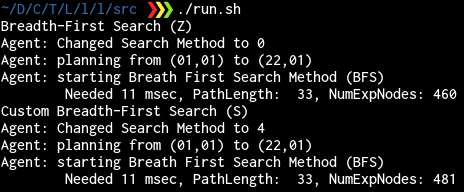
\includegraphics[width=.46\linewidth,scale=1]{./images/lab2_bfs.png} & 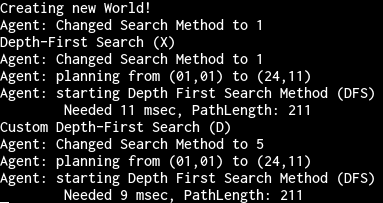
\includegraphics[width=.36\linewidth, scale=1.5]{./images/lab2_dfs.png} \\
      \hspace{0.5cm} (a) & \hspace{0.5cm} (b)
    \end{tabular}
    \caption{Comparison between built-in and custom implementation (a) BFS - (b) DFS \label{fig:BFS and DFS}}
\end{figure}

%\begin{figure}[h]
%    \centering
    %  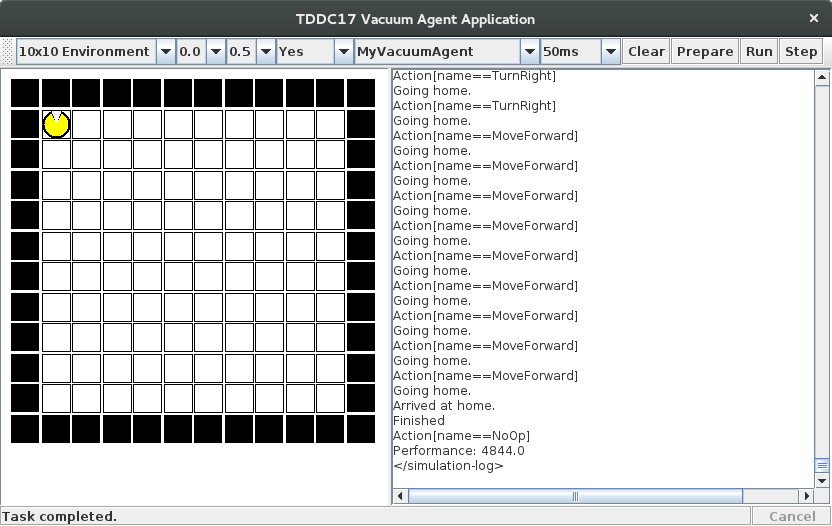
\includegraphics[width=0.83\linewidth]{./images/lab_1.png}
  %  \caption{Screenshot\label{Vacuum cleaner}}
%\end{figure}

\newpage
\thispagestyle{empty}
\section{Theory : questions \\ }

\textit{\textbf{1. In the vacuum cleaner domain in part 1, what were the states and actions? What is the branching factor?}}

In the domain part 1, each square of the grid is a state, which can be clean
or with dirt.The initial state is \textit{In(1,1)}, the starting point in
the grid.The goal state is the position of a square filled with dirt.
In a given state, the possible actions are \textit{suck} and \textit{move} (up,
down, right or left).
The branching factor \textbf{b} is 4 in this domain.

\textit{\textbf{2. What is the difference between Breadth First Search and Uniform Cost Search in a domain where the cost of each action is 1?}}

%We know that BFS is optimal if all step-costs are the same.
%In a domain where the cost of each action is 1, there is no difference between
%BFS and Uniform Cost search because every priority is equal to 1.

In a domain where the cost of each action is 1, the difference between
breadth-first search and uniform-cost search is that BFS stops as soon as it
find the goal. On the other hand, uniform-cost search still examines all the other
nodes at the goal's depth to find a lower cost solution.

\textit{\textbf{3. Suppose that h1 and h2 are admissible heuristics (used in for example A*). Which of the following are also admissible?}}

An admissible heuristic never over estimate the cost to reach the goal from n.
Given that h1(n) and h2(n) are admissible, \textbf{(h1+h2)/2} and \textbf{max (h1,h2)}
are also admissible.

\textit{\textbf{4. If one would use A* to search for a path to one specific square in the vacuum domain, what could the heuristic (h) be? The cost function (g)? Is it an admissible heuristic?}}

An admissible heuristic never overestimates the cost to reach the goal. Therefore
a possible \textbf{h(n)} could be the Manhattan distance between the current node
and the goal node. The cost function \textbf{g(n)} could be the total ammount of step
from the start position to the current node. Given the definition, it would be
an admissible heuristic.

\newpage
\thispagestyle{empty}

\textit{\textbf{5. Draw and explain. Choose your three favorite search algorithms and apply them to any problem domain (it might be a good idea to use a domain where you can identify a good heuristic function). Draw the search tree for them, and explain how they proceed in the searching. Also include the memory usage. You can attach a hand-made drawing.}}

Assuming that we have the following graph, we want to find the shortest path to go
from A to F.

\begin{figure}[h]
    \centering
    \begin{tabular}{cc}
      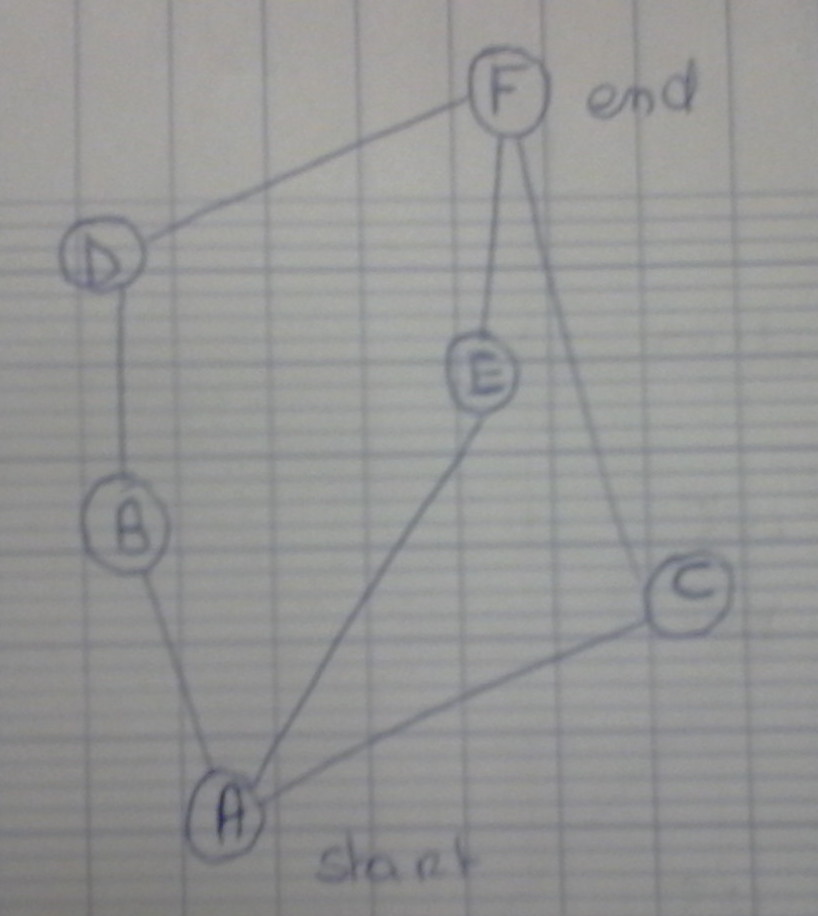
\includegraphics[width=.38\linewidth,scale=1]{./images/graph.jpg} & 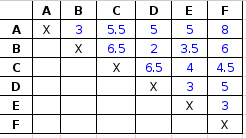
\includegraphics[width=.36\linewidth, scale=1.5]{./images/table.png} \\
      \hspace{0.5cm} (a) & \hspace{0.5cm} (b)
    \end{tabular}
    \caption{Q5 : Sample graph problem (a) Graph - (b) Distance table \label{fig:Graph and table}}
\end{figure}

\paragraph{Breadth First Search}

BFS explores the tree level by level and always expand to the shallowest
node in the frontier.

\begin{figure}[h]
    \centering
    \begin{tabular}{cc}
      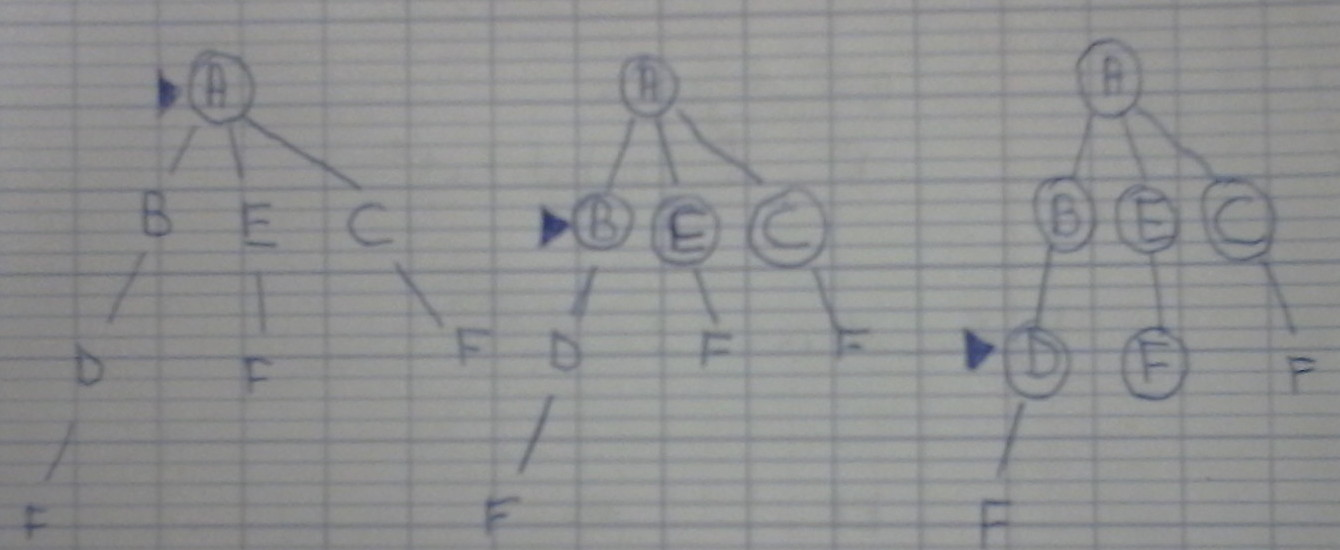
\includegraphics[width=.54\linewidth,scale=1]{./images/bfs.jpg} & 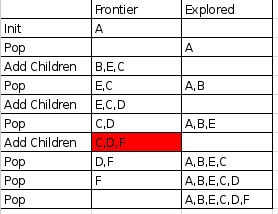
\includegraphics[width=.29  \linewidth, scale=1.5]{./images/bfs_table.jpg} \\
      \hspace{0.5cm} (a) & \hspace{0.5cm} (b)
    \end{tabular}
    \caption{BFS (a) Search - (b) Step table \label{fig:BFS}}
\end{figure}

For each child of the expanded node, BFS tests if this child is not in already
explored or in the frontier. If not it tests if this child state is the goal
state. If this statement is true, it returns the solution.
In this case the algorithm stops just before the red square \textit{Figure 3.b}.

As far as memory is concerned, every node is stored either in the frontier or explored
list. The branching factor \textit{b} is 1$\leq b \leq$3 and the goal depth \textit{d} is 2.
The space complexity $O(b^d) \approx O(3^2)$.

\paragraph{Depth First Search}

DFS explores the tree branch by branch, expanding to the first child node,
deeper and deeper until a goal is found or a node has no children.

\begin{figure}[h]
    \centering
    \begin{tabular}{cc}
      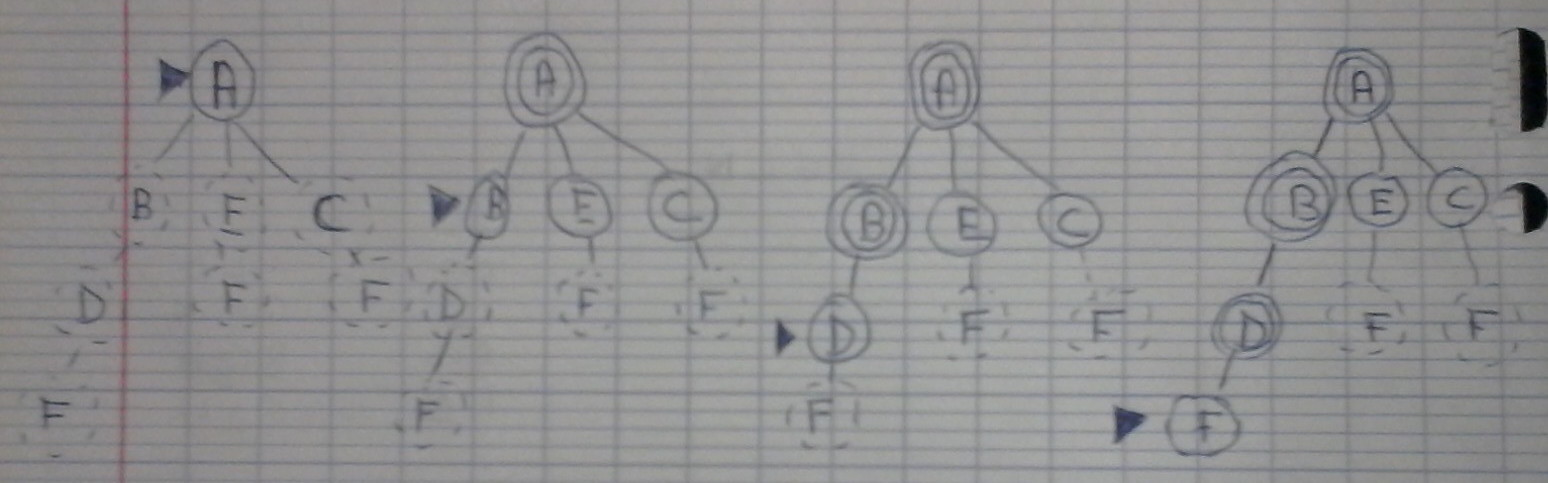
\includegraphics[width=.54\linewidth,scale=1]{./images/dfs.jpg} & 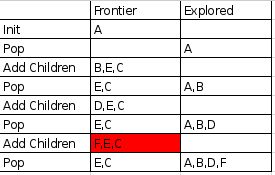
\includegraphics[width=.29  \linewidth, scale=1.5]{./images/dfs_table.png} \\
      \hspace{0.5cm} (a) & \hspace{0.5cm} (b)
    \end{tabular}
    \caption{DFS (a) Search - (b) Step table \label{fig:DFS}}
\end{figure}

We can easly notice that DFS is not optimal, the solution returned \textit{Figure 4}
is not the shortest path : path cost equal to
$3>2$ on the branch A-E-F.

The space complexity is equal to $O(bd) \approx O(3*2)$, which is less than BFS.
\thispagestyle{empty}

\paragraph{A* Search}

This algorithm is based on informed search.
A good heuristic \textit{h(n)} is the straight line between the goal and
the current node. The cost function \textit{g(n)} is the total cost from the start
to the current node.

\textit{Figure 2.b} is used to compute the algorithm. The function
$f(n)=h(n)+g(n)$ after an expansion for each child node to always select the
cheapest path.

\begin{figure}[h]
    \centering
      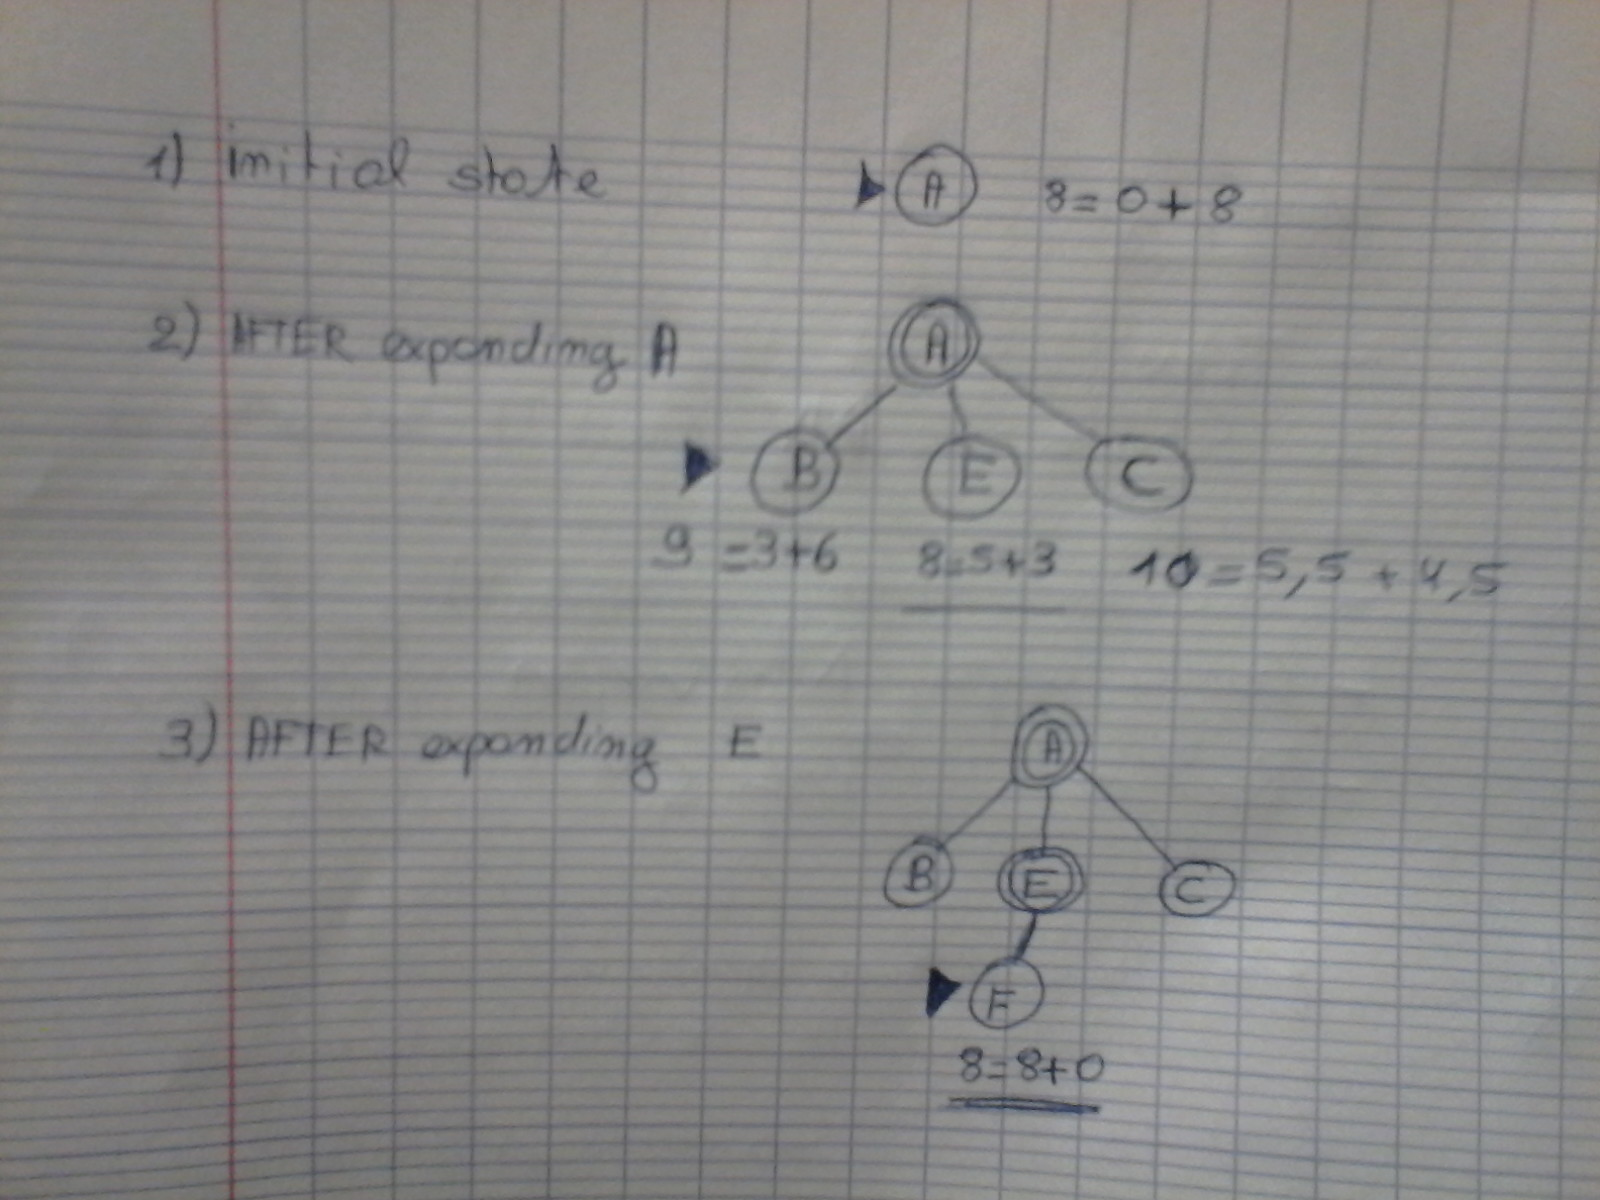
\includegraphics[width=.73\linewidth,scale=1]{./images/astar.jpg} \\
    \caption{A* Search \label{fig:Astar}}
\end{figure}

In the worst case, the space complexity is $O(b^d)$.
\newpage

\textit{\textbf{6. Look at all the offline search algorithms presented in chapter 3 plus A* search.
Are they complete? Are they optimal? Explain why!}}

\paragraph{Breadth First Search}

Breadth first search is complete if the number of node is finite. Indeed all nodes
will be visited, so eventually it will find a solution. However it is only optimal
if the cost of each step is the same because the shallowest node is not always
the least cost solution.

\paragraph{Uniform Cost Search}

Since UCS is based on BFS but with a priority queue instead of the FIFO queue and
expand to the lowest path cost node, it is both complete and optimal.

\paragraph{Depth First Search}

DFS is not complete (Tree Version) is not complete because it can loop infinitely
on one branch and therefore never find a solution. It is also not optimal because it
will always return the first solution found, even if a lower cost solution exists.

\paragraph{Depth-limited search}

The idea is to limit the depth to solves infinite-path problem. However if the goal
is beyond the limit, the algorithm will never return a solution. Therefore it is
not complete.
For the same reasons as DFS, it is also not optimal.

\paragraph{Iterative Deepening Depth First Search}

This algoroithm simply use Depth-limited search but with a increasing depth limit
until a solution is found. Like BFS it is complete if the branching factor b is
finite. It is optimal if each step cost is the same.

\paragraph{Bidirectionnal}

The Bidirectionnal search is only optimal and complete when BFS is used on both side
with all step costs equals. However it is not applicable very often.

\paragraph{A* Search}

A* is complete in finite space but its optimality depends on the chosen heuristic.
If the heuristic is admissible (never overestimates the cost to reach the goal)
 and consistent, it is optimal.

\textit{\textbf{7. Assume that you had to go back and do lab 1 once more, but this time with obstacles. Remember that the agent did not have perfect knowledge of the environment but had to explore it incrementally. Could you still use the search algorithms you have learned to guide the agent's execution? What would you search for? Give an example.}}

If we had to redo lab 1 but with obstacles, we could implement a search algorithm.
However, given that the agent has no knowledge of the environment when it starts,
it would not be possible to use heuristic search. In fact we would have to use
uninformed search algorithms.

The objective of this search would be to cross the world until every square is explored,
and suck the dirt when necessary.

Finally to reach start position, after the environment is fully discovered,
we could use an heuristic algorithm, for example A*.
\thispagestyle{empty}
